\documentclass{rapportECL}
\title{RANDIMBISOAhajanirina38007151} %Titre du fichier

\begin{document}

%----------- Informations du rapport ---------

\titre{Développement Mobile} %Titre du fichier .pdf
\UE{M1 Informatique} %Nom de la UE
\sujet{-} %Nom du sujet

\enseignant{Etienne \textsc{Payet}} %Nom de l'enseignant

\eleves{Hajanirina \textsc{Randimbisoa}} %Nom des élèves

%----------- Initialisation -------------------
        
\fairemarges %Afficher les marges
\fairepagedegarde %Créer la page de garde
\listoffigures  % table des figures
\tabledematieres %Créer la table de matières



%------------ Corps du rapport ----------------


\section{Résumé} 

Pour compléter l'unité d'enseignement développement mobiles, on a choisi de concevoir un jeu pour titre FlyBirds. Ce rapport montre les étapes et démarches que j'ai suivi pour réaliser enfin ce projet. Le travail est sur deux plateforme Android en utilisant le langage JAVA et iOS en utilisant SWIFT. J'ai utilisé AndroidStudio\cite{AndroidStudio} vesion 3.5.2 et Xcode\cite{iOS} version 11 comme outils de développement et overleaf pour la rédaction \cite{Overleaf}.

Selon le cahier de charge et les besoins\cite{Cours}, j'ai utilisé les cours, TD et TP que nous avons appris et fait en classe. Puis j'ai consulté aussi plusieurs tutoriels\cite{OpenClassroom} et forum d'entraides comme stackoverflow\cite{Stackoverflow}, github\cite{Github} pour certains problèmes que j'ai rencontré. Les icônes et fond d'écran utilisés tout au lond de ce projet sont disponibles sur le site de blue flappy Bird sprite\cite{Icon}.
Dans ce rapport,je vais évoquer la structure du projet et sa  réalisation en illustrant avec des captures. Prémièrement sur le plateforme Android puis celui de iOS. Ce projet est libre et opensource, pour le télécharger voici un lien vers le dépôt github\cite{Githubd}.



\section{Introduction}
Ce jeu FlyBirds se concentre sur un jeu de tir entre un chasseur et les oiseaux. Le but principal c'est de tirer sur les oiseaux avant qu'ils ne tuent le chasseur. Ce jeu est très amusant et motivant, grâce à la fonction HighScore, on veut toujours jouer pour battre son propre record.

En terme d'utilisation, il est très simple à manier. Il suffit d'utiliser ses doigts pour glisser vers la gauche ou droite. Le chasseur sous forme avion se déplace et orienté facilement aussi à l'aide du sansor que j'ai utilisé. 


%------------- Commandes utiles ----------------

\section{FlyBirds : Plateforme Android}
\subsection{Architecture générale}
Dans ce répertoire, je vais mentionner quelles sont les classes très importantes et nécessaires. Plus precisement, ce sont les composantes qui présente l'architecture du projet.\newline


a - MainActivity.java

Cette classe MainActivity.java est la classe le plus important et essentielles dans le développement de mon projet. J'ai mis dans cette classe, le menu principal de jeu, le score ainsi que le contrôle de son.

On a la méthode onCreate\cite{AndroidStudio} qui est la création des activités qui va nous permetre de relier l'activité avec la vue avec la méthode setContentView. Puis, on a la méthode findViewById pour récupérer un élément de la vue selon son paramètre. \newline 

b- GameView.java

Cette classe conserve toutes nos fonctions qu'on aura besoin pour le fonctionnement du jeu. Elle hérite le SurfaceView et constitue plusieurs éléments pour déssiner à l'aide de canvas, bitmap et paint. On peut trouver des fonctions comme :
\begin{itemize}
    \item update : quand le chasseur tire sur le prédateur il faut renouveler ses munitions, et on fait un random pour les oiseaux et de changement de vitesse en fonction du score.
    \item draw : pour dessiner les balles, oiseaux et le chasseur.
    \item saveIfHighScore : si on a un nouveau score on fait un update du precedent et on garde le meilleur score.
    \item OnTouchEvent : lorsque on tape ou touche l'ecran, le chasseur se déplace suivant l'orientation indiqué. \newline
\end{itemize}


c - GameActivity

Dans le développement de ce jeu, cette classe est le noyau du jeu. Elle est liée au nombre maximale du boucles, fonctions, la mise en pause, la gestion de l'interruption du jeu et la reprise à l'aide de la méthode onResume. On initialise le GameView dans cette classe pour avoir la vue ou l'interface graphique. Bref, c'est la classe qui va gérer le lancement du jeu. \newline

d - Bird.java

Cette classe contient les parametres pour créer les predateurs, les oiseaux. J'ai crée l'oiseau avec le variable bird en utilisant de Bitmap. C'est dans cette classe que j'ai definit la taille de l'oiseau, la vitesse de l'oiseau. La méthode getCollisionShape est utilisé pour récuper la forme en 2D de l'oiseau. \newline

e - Flight.java

Cette classe assure la création du chasseur et la munition. Comme la création des oiseaux, j'ai utilisé le Bitmap et getCollisionShape pour récupérer la forme de l'avion qui est le joueur. Le shootCounter est utiliser pour faire une boucle de tire. Puis, la méthode getDead récupère le l'avion en 2D cassé, c'est-à-dire, lorsque les oiseaux touchent le chasseur, l'avion se crashe.\newline

f - Bullet.java

Cette classe constitue uniquement la personnalisation et la création des balles. Bitmap pour la création d'image et la Rect getCollisionShape le responsable du retour en 2D. On peut trouver aussi la taille et la largeur de la balle avec les variables width et heigh et l'attribution du son\cite{Son} pour ce dernier. \newline

g - Background.java

Pour avoir une aspect attirante et un décor, c'est dans cette classe que tout cela se passe. Pour definir l'arrière plan du jeu, il y a le bitmap pour decoder le ressource qui n'est autre que le fond\cite{Images}.\newline

h - Geolocalisation

Pour connaître et récupérer la position du joueur, c'est dans cette classe qu'on va définir tout les paramètres\cite{AndroidStudio} dont on a besoin. Pour simplier les choses, j'ai utilisé une fonction qui va accéder à Google Maps afin d'afficher la position réelle du chasseur.\newline

i - Internationalisation

On connaît tous que l'internationalisation d'une application devient presque une obligation si on veut développer un jeu et le mettre dans PlayStore. Pour cela, il suffit de créer un fichier de langue dans le dossier values des ressources (res). Puis, le nom du répertoire devra avoir pour valeur values-fr pour suivre la norme ISO 639-1 d'où l'abréviation "fr".\newline

j - Capture

Pour rendre le jeu interessant, on a ajouté une possibilité de prendre une photo et qui devrait apparaître sur le highscore. Pour être prudent et pour éviter le crash de l'application, on va invoquer une intension de prendre une photo via la méthode StartActivityForResult()\cite{AndroidStudio} afin d'être protéger par la méthode ResolveActivity().

Pour pouvoir enregistrer l'image, on a besoin d'une autorisation de l'utilisation de l'appareil photo via RequestTakePhoto\cite{AndroidStudio} et de stockage getExternalStoragePublicDirectory. Pour ce faire, la lecture et son écriture requièrent ReadExternalStorage et WriteExternalStorage pour le stockage externe. Tout cela devait se passer dans l'android manifest.\newline

\subsection{Illustration des codes}

a - MainActivity.java

\insererfigure{logos/MainActivity.png}{10cm}{Classe MainActivity}{Label de la figure}

b - GameView.java 

\begin{center}
    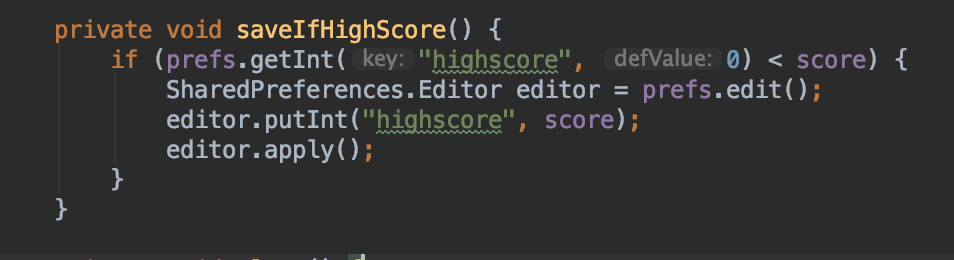
\includegraphics[scale = 0.5]{logos/GameView.png}
    \captionof{figure}{Sauvegarde highScore dans GameView}
\end{center}

c - Bird.java

\begin{center}
    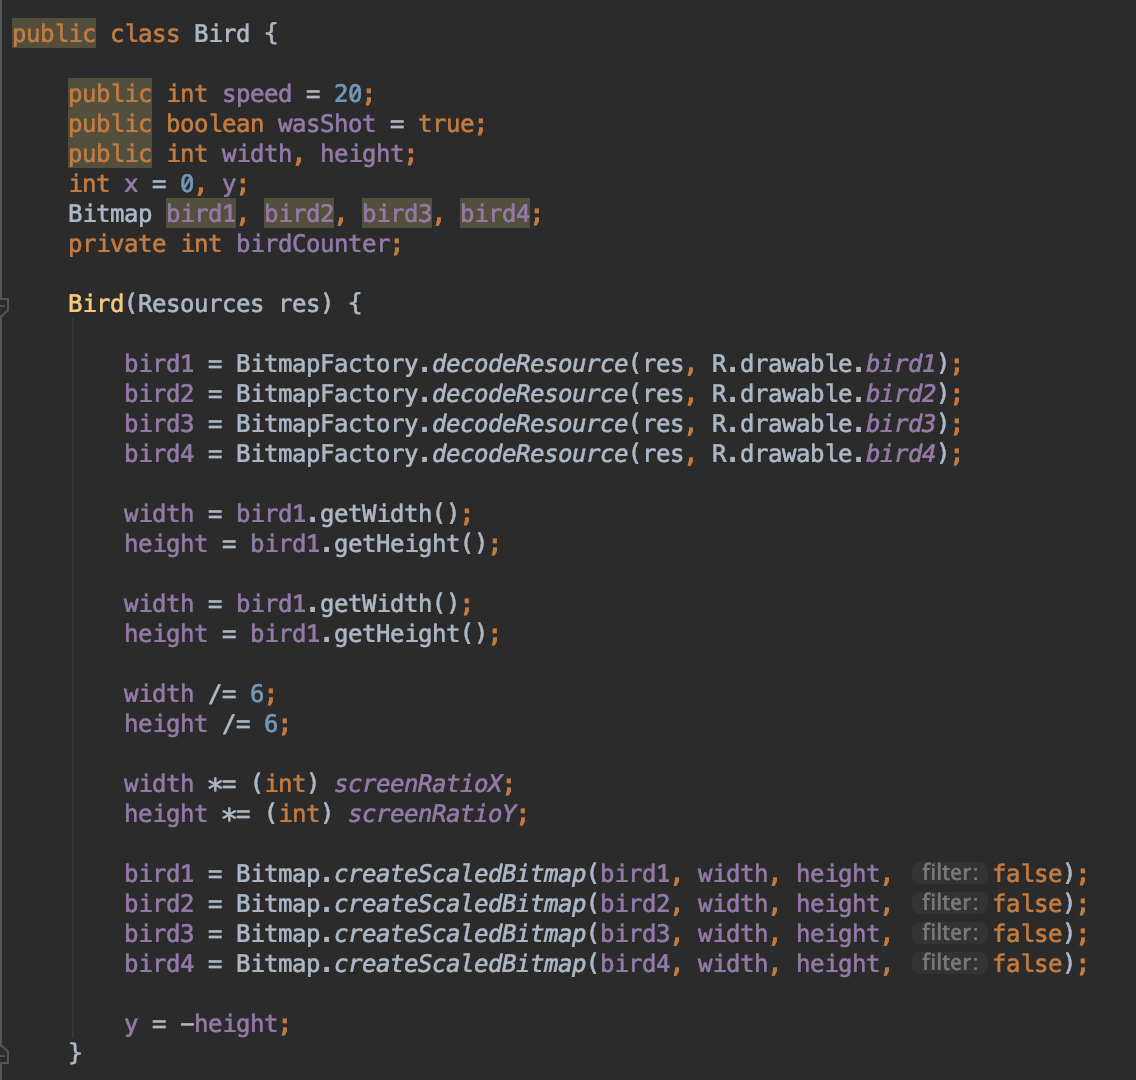
\includegraphics[scale = 0.5]{logos/Bird.png}
    \captionof{figure}{Création de la classe Bird}
\end{center}

d - Flight.java

\begin{center}
    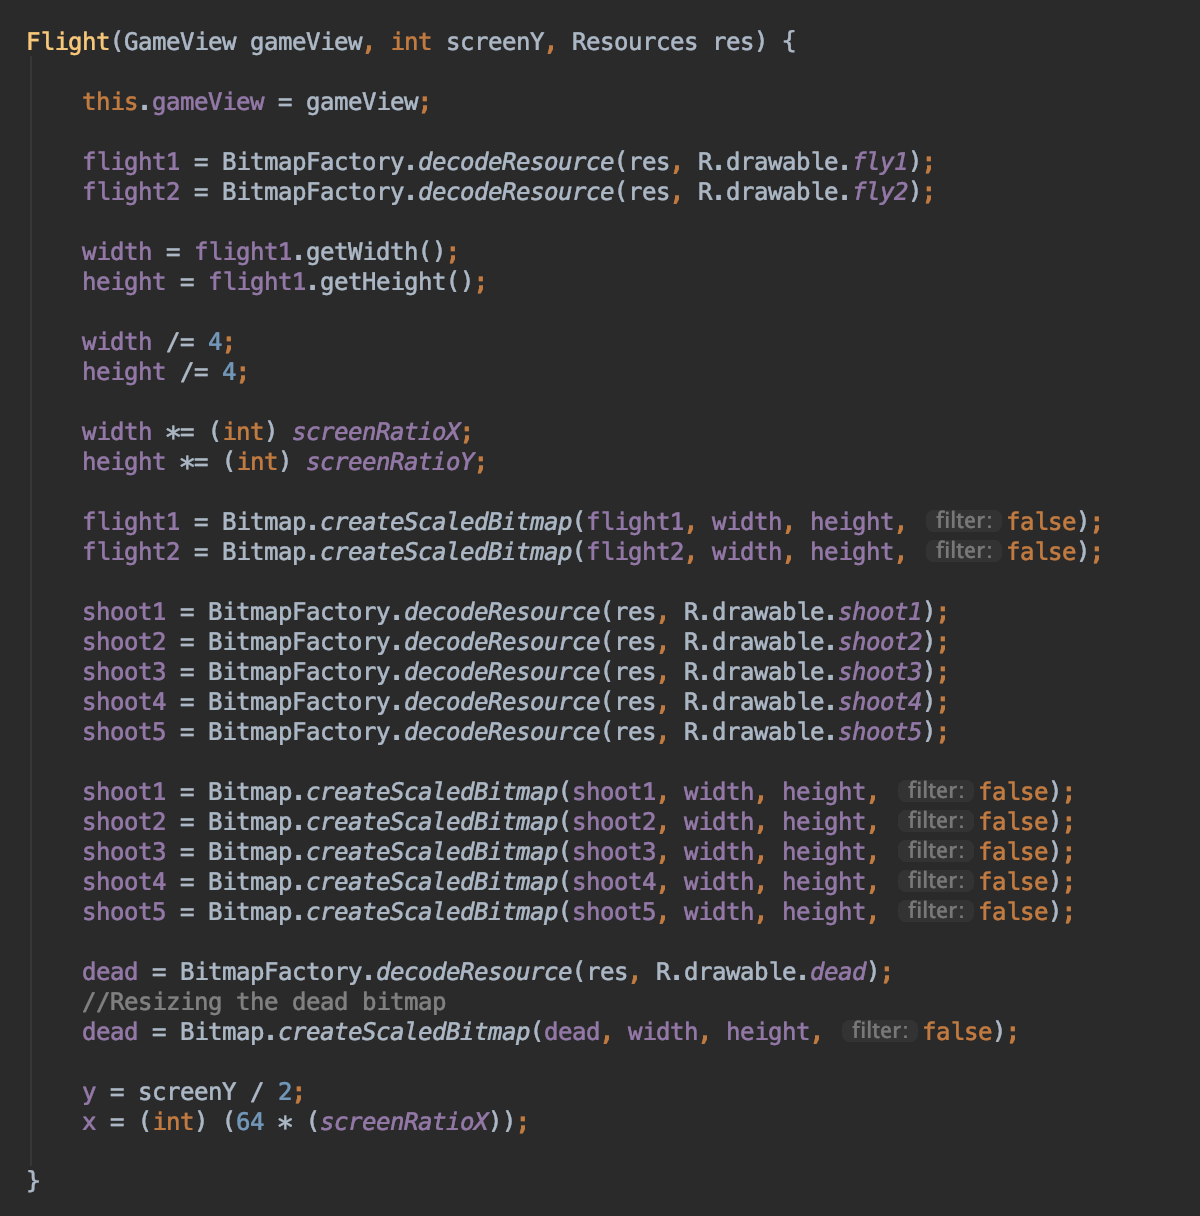
\includegraphics[scale = 0.5]{logos/Flight.png}
    \captionof{figure}{Classe Flight}
\end{center}

e - Bullet.java

\begin{center}
    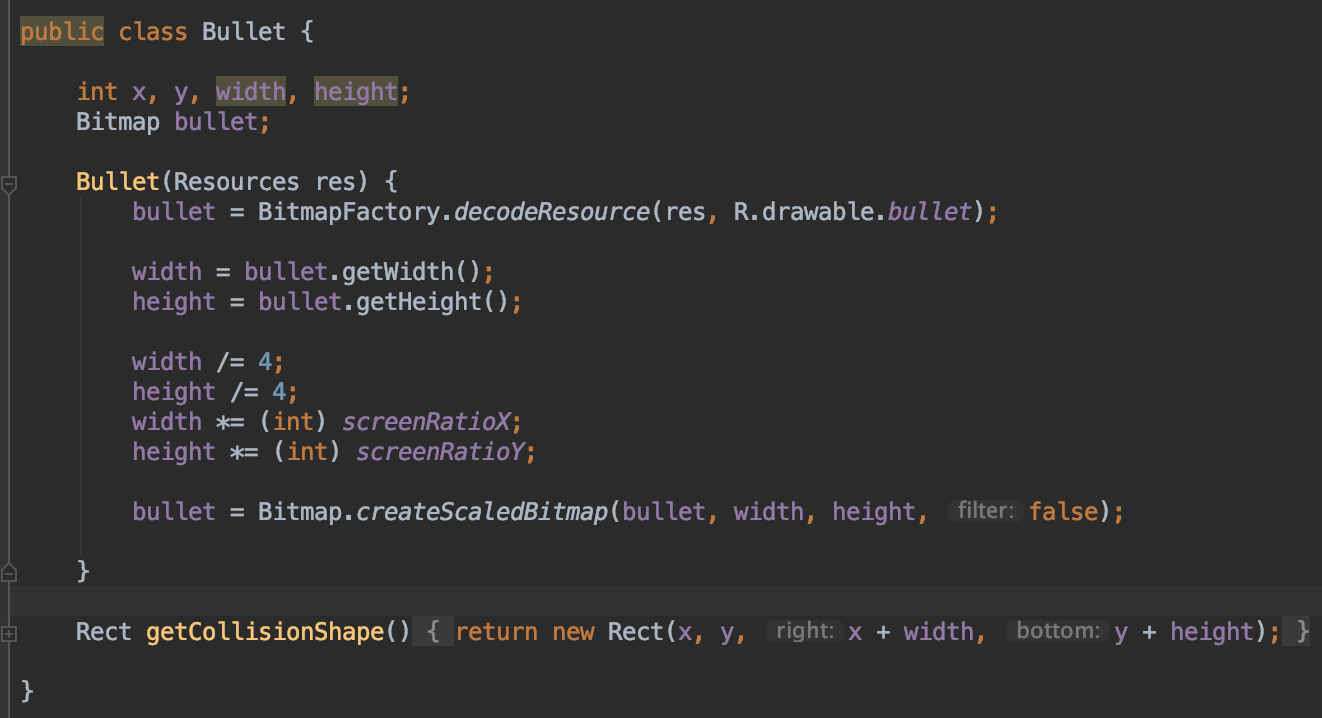
\includegraphics[scale = 0.5]{logos/Bullet.png}
    \captionof{figure}{Création des munitions}
\end{center}
f - camera

\begin{center}
    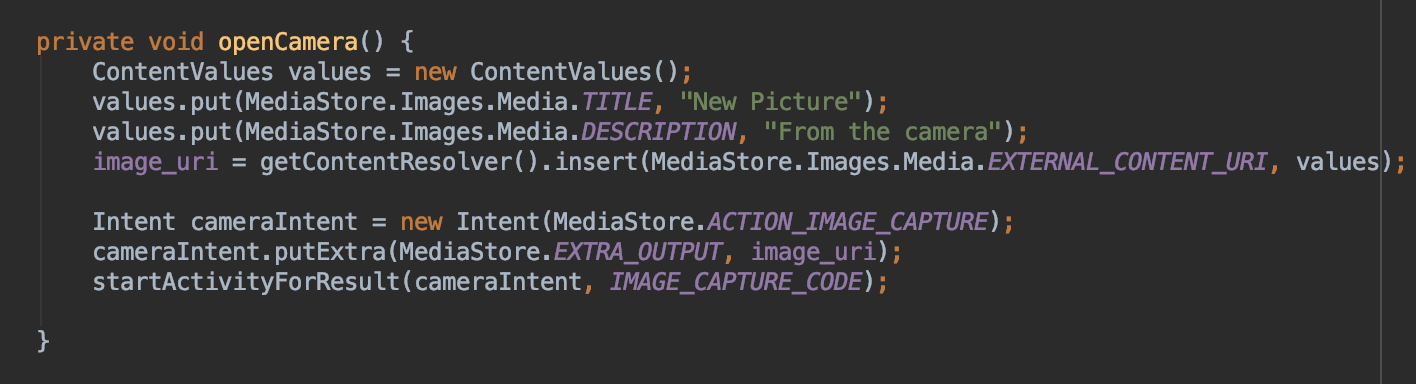
\includegraphics[scale = 0.5]{logos/camera.png}
    \captionof{figure}{Fonction du capture}
\end{center}


\section{FlyBirds : Plateforme iOS}
\subsection{Architecture générale}
On trouve dans cette partie la présentation de l'architecture générale de la version iOS du projet. Comme j'ai mentionné au le début, l'outil que j'ai utilisé c'est l'Xcode\cite{xCode} 11. J'ai fait un choix entre Unity et SpriteKit\cite{Spritekit} pour accompagner SWIFT et j'ai choisi SpriteKit. C'est simple à utiliser pour un débutant et qui se concentre sur l'écosystème d'Apple.


Cela nous donne une certaine confiance dans le fait que tous les nouveaux produits d'Apple seront bien pris en charge. Par exemple, on peut utiliser le même code SpriteKit\cite{Spritekit} pour que notre jeu fonctionne sur iOS, macOS et tvOS sans accroc.\newline

a - GameScene.swift

Cette classe est la résponsable principale de notre jeu. Elle contient l'ensemble du jeu. Elle comporte aussi des fonctions utiles pour manier le jeu et le geste courant ainsi la double tap.


b - GameViewController.swift

Le GameViewController.swift va nous permettre de lancer la vue en appelant la GameScene.swift. On peut voir la fluidité de jeu aussi en utilisant la méthode showsFPS.\newline


c - Internationalisation

Localizable.strings est utilisé pour gérer l'internationalisation du jeu. Pour avoir la traduction, dans le cas dans ce jeu, francais en anglais, on utilise la KeyValues.\newline


d - Géolocalisation

Comme on a fait sur Android, pour localiser la position du joueur, Geolocalisation.swift est utilisé pour faire cela et en utilisant la méthode CCLocationManager\cite{GooglemapsiOS}. Chez Apple\cite{iOS}, ce fichier fait appel à une classe qui s'appelle MKMapView qui le responsable d'affichage de la carte sur l'ecran de user.



\subsection{Illustration des codes}
 a - GameScene
 
 \begin{center}
    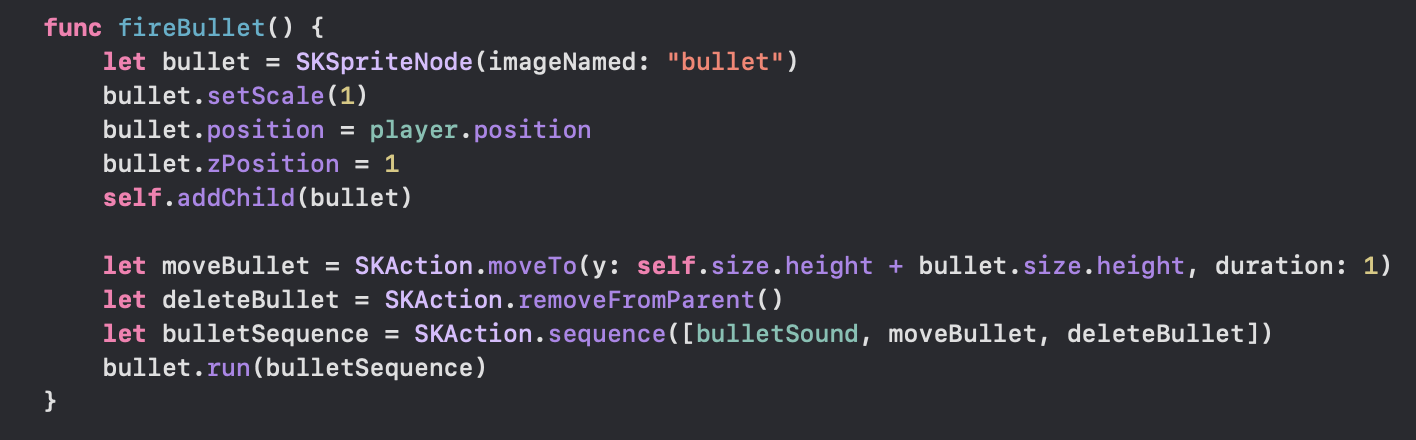
\includegraphics[scale = 0.5]{logos/FireBullet.png}
    \captionof{figure}{Création des munitions}
\end{center}

 b - GameViewController
 
 \begin{center}
    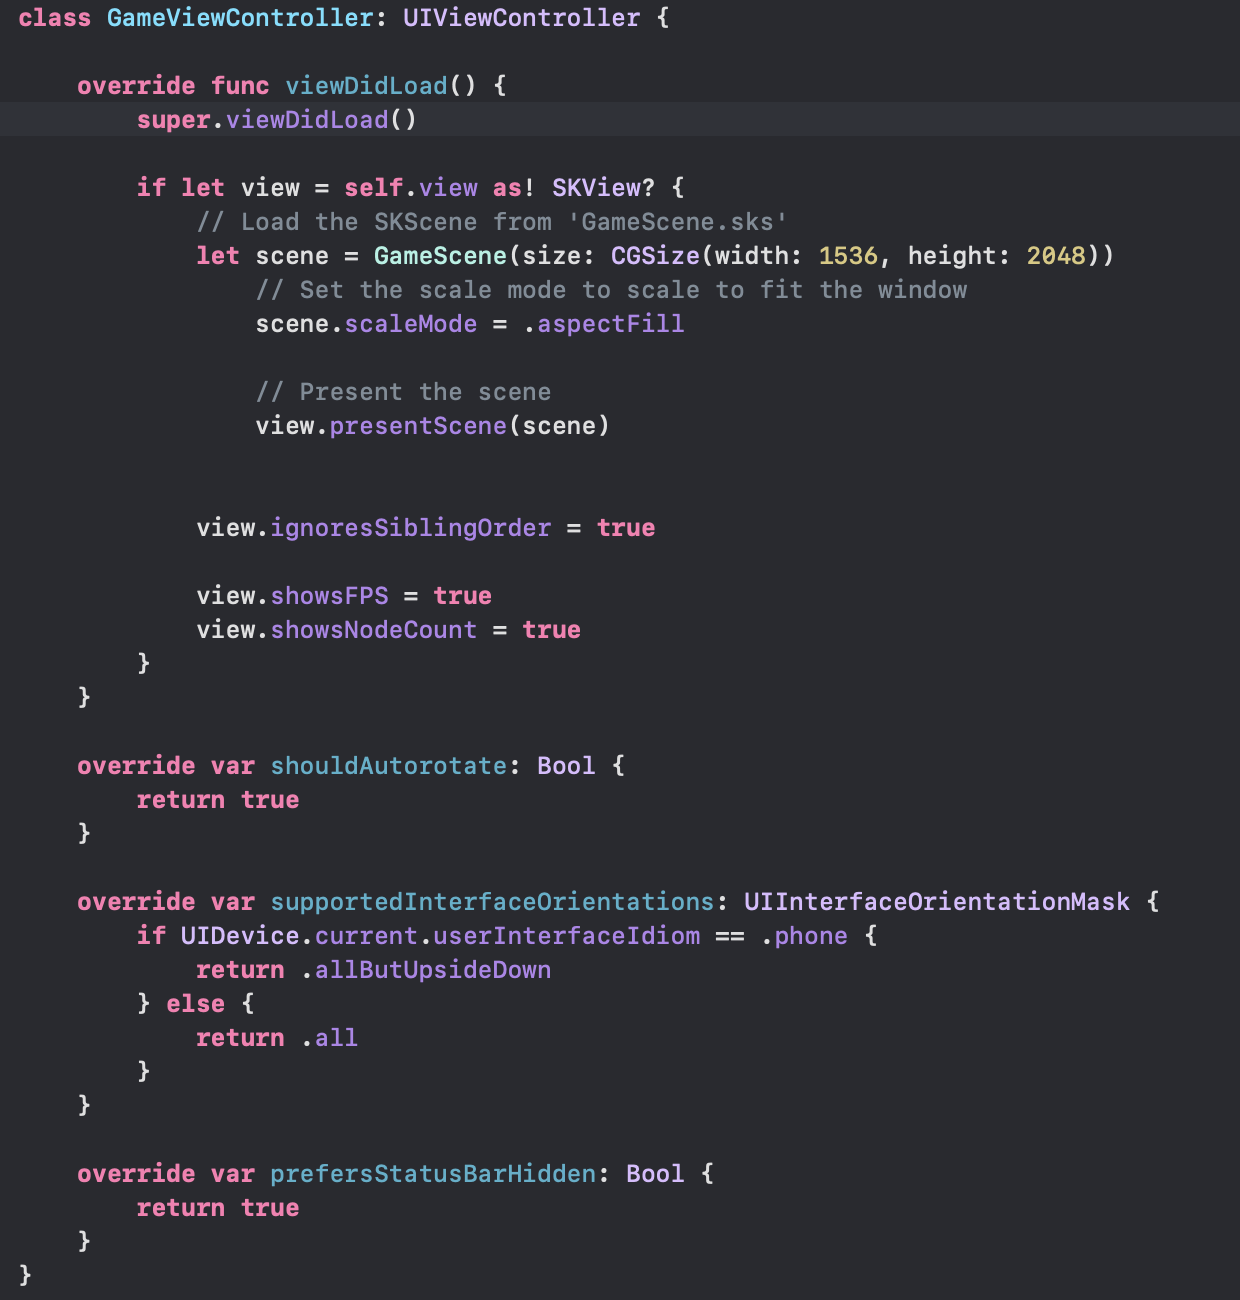
\includegraphics[scale = 0.5]{logos/GameViewController.png}
    \captionof{figure}{Classe GameViewController}
\end{center}

\newpage
\section{Résultats}
\subsection{Android}
a - Accueil

Voici donc à quoi ressemble l'écran principal du jeu : 

\begin{center}
    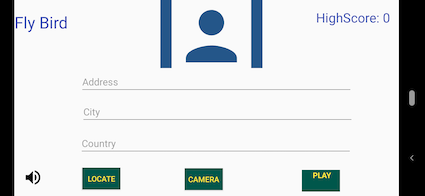
\includegraphics[scale = 0.5]{logos/accueil.png}
    \captionof{figure}{Accueil v2.0 }
\end{center}

b - Mode Jeu

Capture en plein jeu : 

\begin{center}
    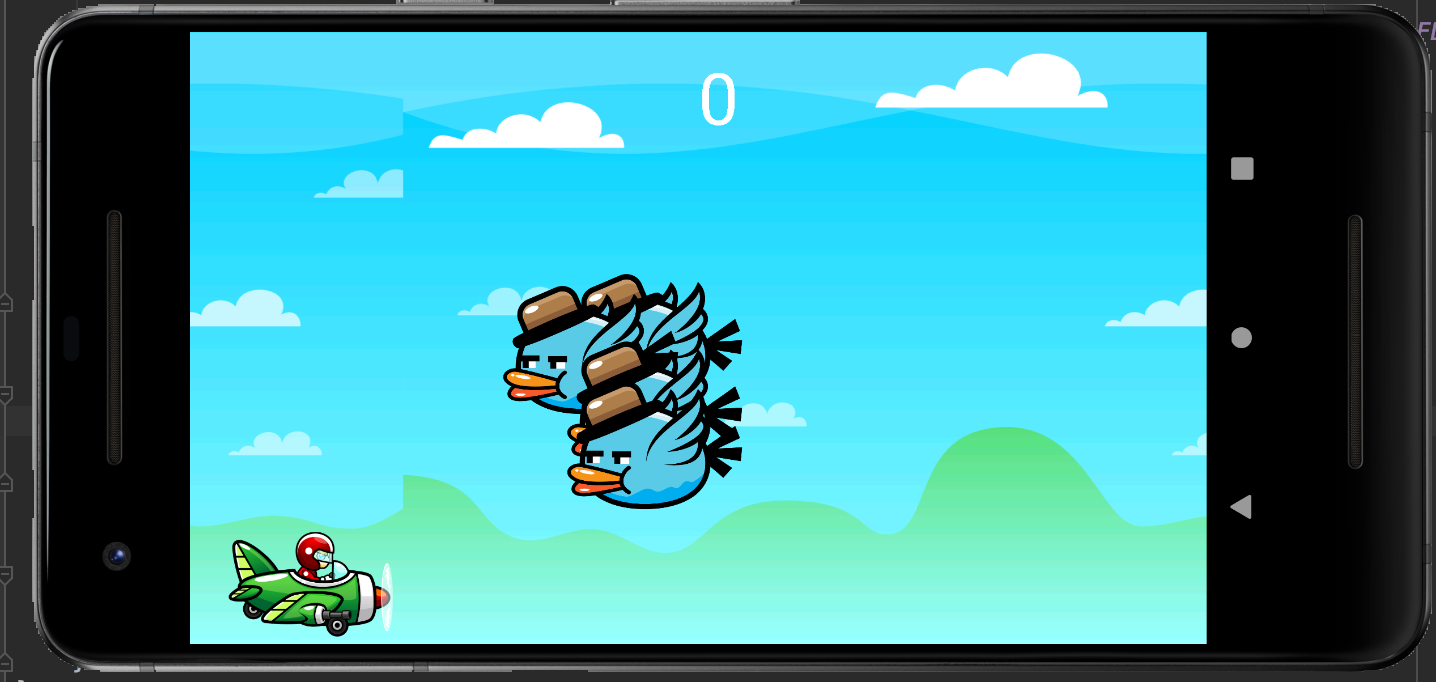
\includegraphics[scale = 0.5]{logos/ModeGame.png}
    \captionof{figure}{Capture en plein jeu android v1.0}
\end{center}

C - Double tap

Lorsqu'on fait un double tap sur l'ecran, il y a un message qui indique l'apropos du jeu : 

\begin{center}
    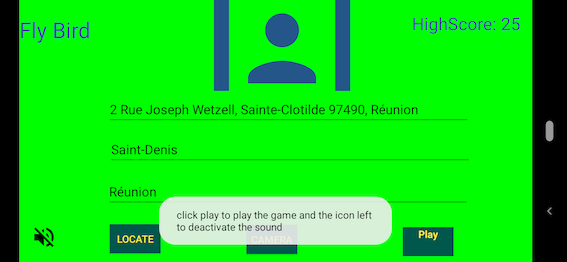
\includegraphics[scale = 0.5]{logos/doubletap.png}
    \captionof{figure}{Double tap}
\end{center}

d - Localisation

J'ai utilisé LocationManager pour afficher et récuperer l'adresse ou l'endroit exacte du joueur: 

\begin{center}
    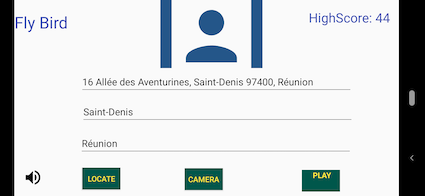
\includegraphics[scale = 0.5]{logos/geolocalisation.png}
    \captionof{figure}{Double tap}
\end{center}

e - Problème rencontré

Dans la partie Android, j'ai eu de difficulté sur la mise en place de la géolocalisation avec la gestion de key maps. En effet, ça ne m'empêcha pas de creuser et trouver des solutions pour résoudre ce problème en utilisant les TP, support de cours et les liens utiles\cite{Cours} qu'on nous a donné en classe.

\newpage
\subsection{iOS}
a - accueil

Pour celui de iOS, j'ai varié un peu le style de l'affichage : 

\begin{center}
    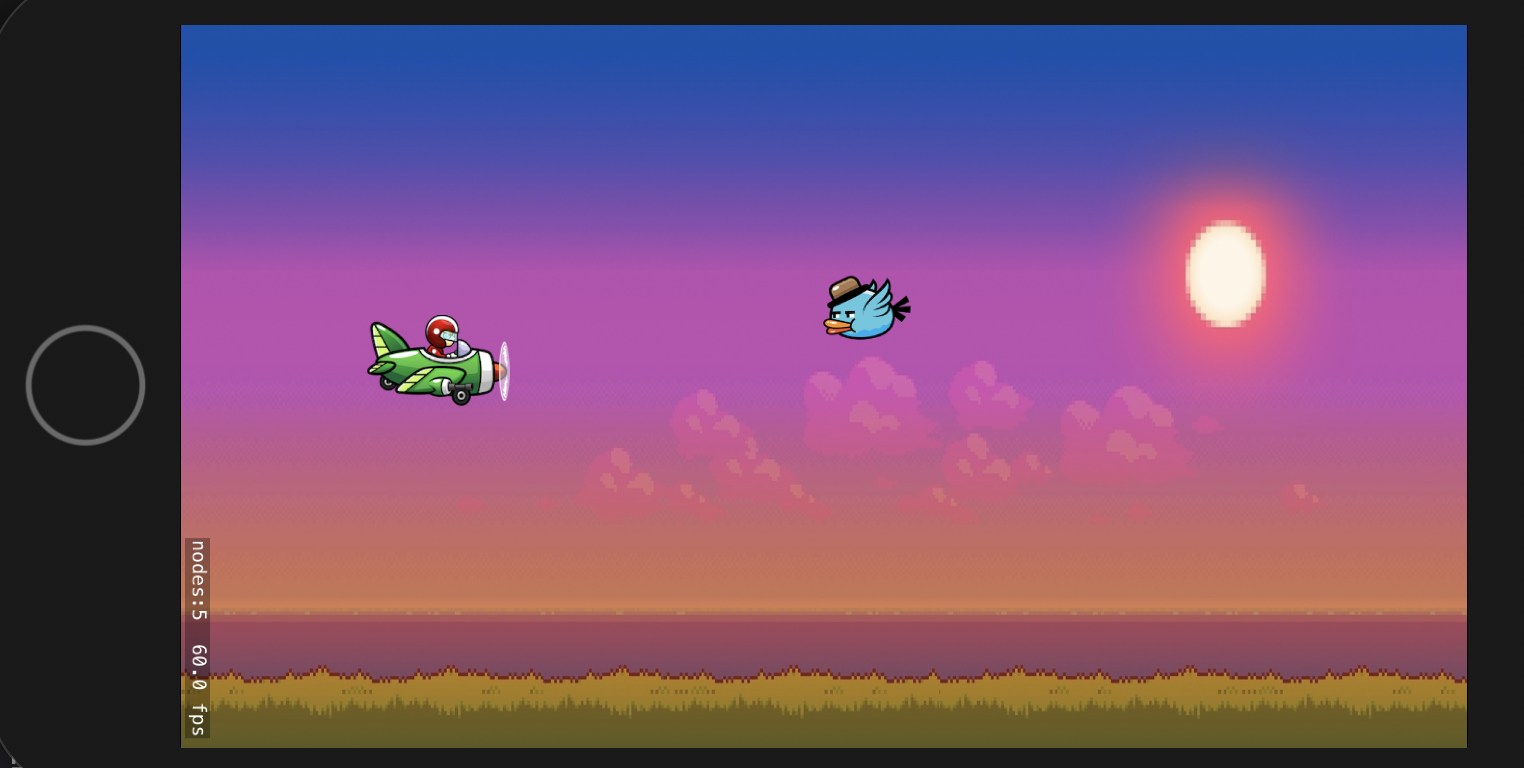
\includegraphics[scale = 0.5]{logos/JeuiOS.png}
    \captionof{figure}{Acceuil du jeu v1.0 }
\end{center}

b - Mode Jeu

Voilà se qui s'affiche à l'écran quand on joue : 

\begin{center}
    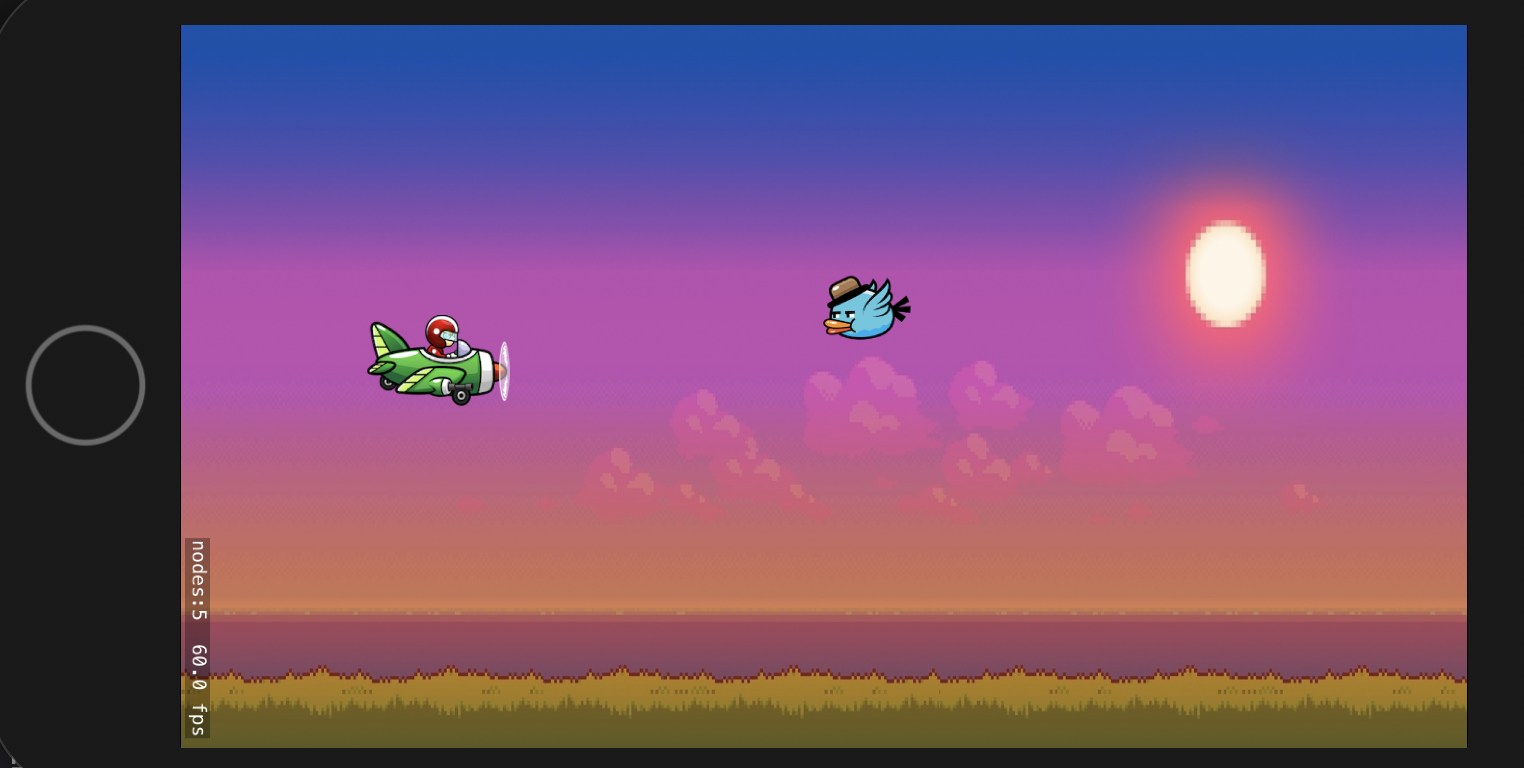
\includegraphics[scale = 0.5]{logos/JeuiOS.png}
    \captionof{figure}{Mode jeu v1.0}
\end{center}

C - Problème rencontré

Dans cette partie iOS, je n'ai pas eu l'occasion de tester l'appareil photo sur un téléphone. Vue que, Apple ne permet pas  l'utilisation de camera sur le simulateur, je ne sais pas si ca fonctionne vraiment ou pas. Pareil pour le géolocalisation. Malgré tout, le projet est presque terminé et quasi-répond au besoins du cahier de charge.

\newpage
\section{Conclusion}

En guise de conclusion, ce projet fut une belle épreuve qui m'a permis plusieurs expérience dans le développement d'applications mobiles que ce soit en Android ou en iOS.

En réalisant ce projet, j'ai rencontré un peu de difficulté au niveau du langage SWIFT\cite{iOS} et l'utilisation de LATEX\cite{Overleaf}. Heureusement que j'ai eu l'occasion de consulter des forums d'aides et on m'a aidé à surmonter les épreuves. Ce n'est pas tout, j'ai aussi le privilège de consulter les TD et l'ensemble des TP qu'on avait fait en cours. Ce projet m'a permis donc d'améliorer mes capacités que ce soit au niveau de la rédaction en LATEX\cite{Overleaf} ou en développement mobiles.
\newpage

\bibliographystyle{unsrt}
\bibliography{bibli}
% mon fichier de base de données s'appelle bibli.bib
\end{document}
